\chapter{映像伝送システム}
\label{chap:video-transmission}

本章では、映像伝送システムを構成する技術要素の仕組みについて解説する。
% \ref{chap:network-transmission}章で必要な、
% それぞれ、○○について述べる

\section{ビデオカメラ}
\label{sec:camera}

% ここはaomさんの引用なので適切にする
ビデオカメラは、映像の入力機構である。
撮影素子であるイメージセンサは、多数の受光素子によって構成されており、それぞれの受光素子は、光エネルギーの明暗に従い電荷を発生する。
撮影対象部から反射される光をカメラのレンズを通して、この撮影素子の受光部にあてることで、その明暗を電荷量を光電変換する。
変換された電圧値を順次読み出し,電気信号に変換することでアナログ値である光情報をデジタル値に変換する。

ビデオカメラによる出力インターフェースとしては、デジタル信号としてはSDIやHDMIのインターフェースを使用するのが一般的である。

\section{ディスプレイ}
\label{sec:display}

% ここはaomさんの引用なので適切にする
ディスプレイは、映像の表示機構である。
ディスプレイには大まかに、アナログディスプレイとデジタルディスプレイに二分できる。

アナログディスプレイでは、CRT、すなわちブラウン管を用いた描画方式である。
管面全体を走査線とよぶ固定パターンでスキャンしつつ、映像信号の輝度成分に従って電子ビームの強さを変調して描画する。
このように、画面上の任意の点の明るさを制御することにより画像を作り上げている。

一方、デジタルディスプレイでは、薄い板状の液晶パネルを用いた描画方式である。
偏光フィルタから入ってきた光を、電極によりピクセルのカラーごとに電荷をかけることにより、配向膜を光が通り抜け描画する。
ブ゙ラウン管の走査方式を後継しており、映像の制御信号として、水平同期信号と垂直同期信号が使われている。

\section{インターレース}
\label{sec:interlace}

画像伝送において、データレートを増やさずに描画回数を増やす技術である。
この方式の特徴は、「人間の視野は動くものの細部を捉えられない」という性質に基づいている。
飛び越し走査とも呼ばれ、奇数番目の走査線を先に送り、偶数番目の走査線をその後に送る。

デジタル化が進んでいる現在でも、走査線を1ラインに割り当てられたものとして、データレートを減らす際の手段として利用されている。
主な例として、日本のテレビジョン放送では、アナログテレビ放送、デジタルテレビ放送のどちらでも使われている。

幸いなことに、4K・8K映像ではインターレース方式は使われることはない。[要出典]
% 幸いな理由と出典先を明示する

\section{色空間と色深度}
\label{sec:colorspace}

一般的に液晶ディスプレイでは、1ピクセルを赤、緑、青、すなわちRGBの3つの色信号で表現する。
多くのPCやゲーム機の出力ではRGBの色空間が使われ、RGBそれぞれ8bit、1ピクセルあたり24bitで表現する。
1ピクセルあたりを表現するビット数を色深度といい、色解像度、色分解能とも言われる。
24bitの色深度では、16,777,216色を表現することができる。

一方、ビデオカメラでは、輝度信号Yと、2つの色差信号を使って表現される色空間であるYUVが使われるが多い。[要出典]
この方式の特徴は、「人間の目は明るさの変化には敏感だが、色の変化には鈍感である」という性質に基づいて、色度信号の情報量を減らすことができるという点にある。

\begin{figure}[htbp]
    \begin{center}
        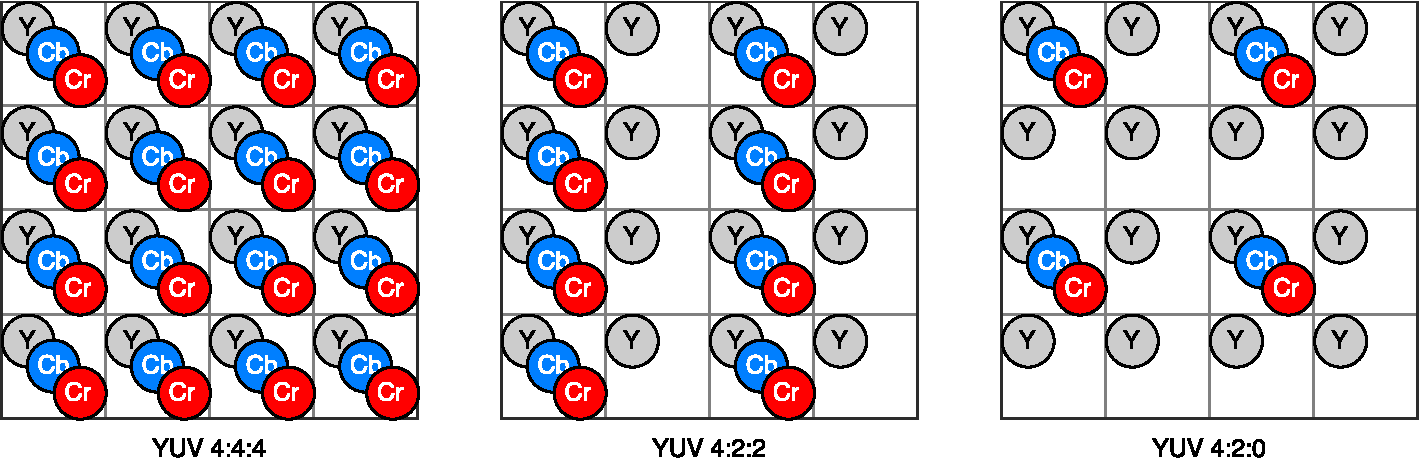
\includegraphics[bb=0 0 681 222,width=14cm]{img/yuv-pixel-structure.pdf}
    \end{center}
    \caption{YUVのピクセルあたりの色情報の構造}
    \label{fig:yuv-pixel-structure}
\end{figure}

% YUVのピクセルあたりの色情報の構造を、図\ref{fig:yuv-pixel-structure}に示す。

YUV 4:4:4では、輝度信号、色差信号共に1ピクセル毎である。
YUV 4:2:2では、輝度信号は1ピクセル毎、色差信号は2ピクセル毎であり、同じ色深度のYUV 4:4:4と比べ、帯域はおよそ2/3となる。
YUV 4:2:0では、輝度信号は1ピクセル毎、色差信号は4ピクセル毎であり、同じ色深度のYUV 4:2:2と比べ、帯域はおよそ3/4となり、同じ色深度のYUV 4:4:4と比べ、帯域はおよそ1/2となる。

なお、図\ref{fig:yuv-pixel-structure}で示した、UV成分であるCb、Crの色のサンプリング方法は、伝送方式の規格によって定められている。

\section{帯域}
\label{sec:bandwidth}
% この部分はあとで何処かに持っていく予定

帯域は解像度の他にも、インターレース、色空間、色深度により変化する。
また、伝送するインターフェースの規格によっても、若干の違いがあるため、ここではHDMIを基準とする。
色深度を8bitとした場合の解像度、フレームレート、色空間別に見たピクセルクロック、帯域を、表\ref{tb:video-bandwidth}に示す。

% 1920x1080p/60 2200x1125 148.5 SMPTE 274M
% 1Channel = 2200 * 1125 * 3 * 8 * 60 * 1.25/3

\begin{table}[htbp]
  \caption{解像度、フレームレート、色空間による帯域の変化}
  \label{tb:video-bandwidth}
  \begin{center}
  \begin{tabular}{c|c|c|c|c|c}
    \hline
    解像度     & フレームレート & 色空間  & ピクセルクロック & 帯域     & 同期区間を含んだ帯域 \\\hline\hline
    3840x2160 & 60p          & RGB    & 148.5MHz      & XX Gbps & YY Gbps           \\\hline
    3840x2160 & 60p          & YUV422 & 148.5MHz      & XX Gbps & YY Gbps           \\\hline
    3840x2160 & 60p          & YUV420 & 148.5MHz      & XX Gbps & YY Gbps           \\\hline
    3840x2160 & 30p          & RGB    & 148.5MHz      & XX Gbps & YY Gbps           \\\hline
    3840x2160 & 30p          & YUV422 & 148.5MHz      & XX Gbps & YY Gbps           \\\hline
    1920x1080 & 60p          & RGB    & 148.5MHz      & XX Gbps & YY Gbps           \\\hline
    1920x1080 & 60p          & YUV422 & 148.5MHz      & XX Gbps & YY Gbps           \\\hline
    1920x1080 & 60i          & RGB    & 148.5MHz      & XX Gbps & YY Gbps           \\\hline
    1920x1080 & 60i          & YUV422 & 148.5MHz      & XX Gbps & YY Gbps           \\\hline
  \end{tabular}\end{center}
\end{table}

\section{インターフェース}
\label{sec:interface}

\subsection{VGA}
VGA(Video Graphics Array)は、IBMが発表したアナログ映像信号の伝送規格、または、同社が開発したVGA表示回路用のチップのことを指す。
DE-15コネクタを使用し、赤、緑、青、垂直同期、水平同期の5つのアナログ信号で映像を伝送することができる。
DDC(VESA Display Data Channel)信号を使用することで、接続機器の対応する解像度を送信することができ、最近では1080pの映像を伝送する機器も多い。
PCでの映像出力方式として普及したが、アナログ信号であることや、音声伝送の手段が別途必要となるため、HDMIやDisplayPortなどのインターフェースに移行が進んでいる。

\subsection{DisplayPort}
DisplayPortは、VESA\footnote{Video Electronics Standards Association ビデオ周辺機器に関する業界標準化団体}によって標準化された映像伝送規格であり、主に超解像度向けのインターフェースとして普及している。
DisplayPort 1.3からは、32.4 Gbpsのデータレートに対応し、8K映像の伝送にも対応している。

\subsection{DVI}
DVI(Digital Visual Interface)は、\footnote{Video Electronics Standards Association ビデオ周辺機器に関する業界標準化団体}によって標準化された デジタル映像信号の伝送規格。
物理層としてTMDS(Transition Minimized Differential Signaling)を使用しており、赤、緑、青、クロックの4つのツイストペアケーブルで構成される。
% TMDSの解説画像

\subsection{HDMI}
HDMI(High-Definition Multimedia Interface)は、映像、音声をデジタル信号で伝送する通信インターフェースの規格である。
DVIを基に、音声伝送機能や著作権保護機能を加えたものであり、物理層はDVIと同じTMDSを使用している。
HDMI 2.0では、帯域を18Gbpsに拡大し、4K@60pに対応している。
% また、HDMI 2.0
% 1.4 / 2.0

HDMI 2.0からは、YCbCr 4:2:0方式によるピクセルエンコーディングの規格が追加され、1/2のデータレートで転送することが可能となった。

\begin{table}[htbp]
  \caption{HDMI 1.4と2.0での4K(3840x2160)映像の対応状況}
  \label{tb:video-bandwidth}
  \begin{center}
  \begin{tabular}{c|c|c|c}
    \hline
      フレームレート & ピクセルあたりの色深度 & HDMI 1.4 & HDMI 2.0\\\hline\hline
    \multirow{4}{*}{30Hz} &
        24bit & 対応   & 対応 \\\cline{2-4}
      & 30bit & 対応   & 対応 \\\cline{2-4}
      & 36bit & 対応   & 対応 \\\cline{2-4}
      & 48bit & 非対応 & 対応 \\\hline
    \multirow{4}{*}{60Hz} &
        24bit & 非対応 & 対応  \\\cline{2-4}
      & 30bit & 非対応 & 対応  \\\cline{2-4}
      & 36bit & 非対応 & 対応  \\\cline{2-4}
      & 48bit & 非対応 & 非対応 \\\hline
  \end{tabular}\end{center}
\end{table}

HDMI 1.4\cite{hdmi-spec-1-4}では、RGB、YCbCr 4:4:4、YCbCr 4:2:2の色空間がサポートされており、HDMI 2.0\cite{hdmi-spec-2-0}では、新たに4K解像度向けのYCbCr 4:2:0がサポートされた。

% また、YCbCr方式

% すなわち、\ref{sec:colorspace}章では、色深度
\begin{figure}[htbp]
    \begin{center}
        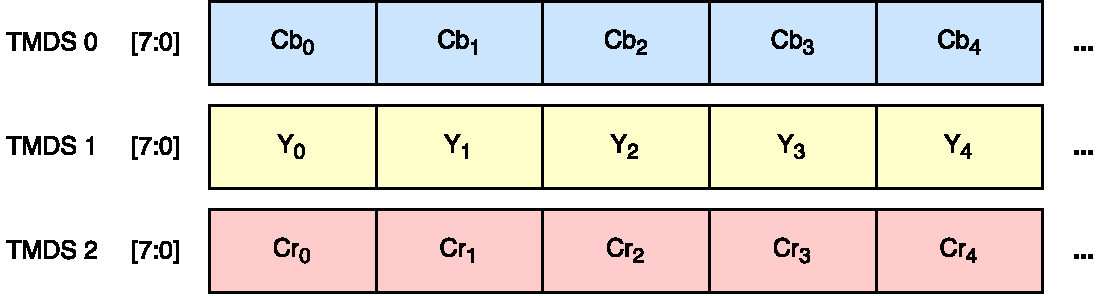
\includegraphics[bb=0 0 531 141,width=13.926cm]{img/hdmi-spec-yuv-444.pdf}
    \end{center}
    \caption{HDMI 1.4 で定義されている YCbCr 4:4:4 方式におけるTMDSマッピング}
    \label{fig:hdmi-spec-yuv-444}
\end{figure}

\begin{figure}[htbp]
    \begin{center}
        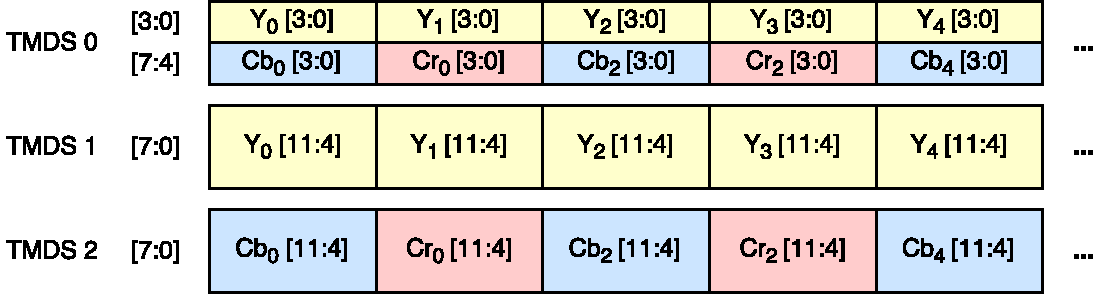
\includegraphics[bb=0 0 531 141,width=13.926cm]{img/hdmi-spec-yuv-422.pdf}
    \end{center}
    \caption{HDMI 1.4 で定義されている YCbCr 4:2:2 方式におけるTMDSマッピング}
    \label{fig:hdmi-spec-yuv-422}
\end{figure}

\ref{sec:colorspace}節では、同じ色深度の場合YUV 4:2:2はYUV 4:4:4と比べ2/3となると述べたが、HDMI 1.4で定義されているYCbCr 4:2:2では、1ピクセルあたりの色深度は変わらず、YおよびCbCrのサンプリング解像度が8bitから12bitになる。
そのため、HDMIでは色空間のYCbCr 4:4:4、YCbCr 4:2:2のどちらであっても帯域には影響しない。

\begin{figure}[htbp]
    \begin{center}
        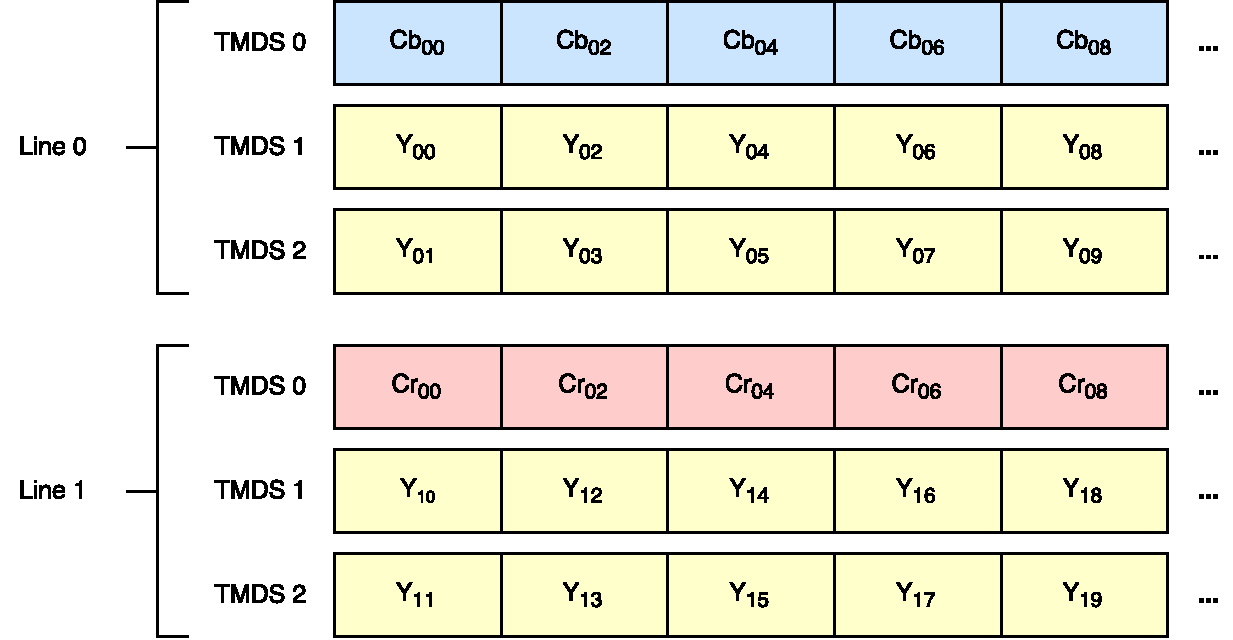
\includegraphics[bb=0 0 591 306,width=15.5cm]{img/hdmi-spec-yuv-420.pdf}
    \end{center}
    \caption{HDMI 2.0 で定義されている YCbCr 4:2:0 方式におけるTMDSマッピング}
    \label{fig:hdmi-spec-yuv-420}
\end{figure}

HDMIでは、24bitの他に、30bit、36bit、48bitの色深度に対応しているが、YCbCr 4:2:0では、24bitのみの対応である。

\subsection{SDI}

SDI(Serial Digital Interface)は、SMPTE\footnote{米国映画テレビ技術者協会}によって標準化された映像伝送規格であり、主に業務機器向けの規格である。

同軸ケーブルを使用しているため、HDMIと比べて距離に対する減衰が少なく、HD-SDIでは、およそ100m遠方に伝送することができる。
BNC端子を使用することが一般的であり、抜け落ち防止のためのロック機能がるため、中継現場で活躍する。

解像度や帯域に応じて、SD-SDI、HD-SDI、3G-SDI、6G-SDI、12G-SDIなど複数の規格が定められている。
また、4K・8K映像を伝送するために、HD-SDIを4本1組で使用して伝送する事も可能である。

% \section{伝送手法}

% \section{まとめ}

% あ
